%cc/cv de overleaf.com :s
\documentclass{beamer}
\usetheme{Frankfurt}
\usecolortheme{seahorse}
\title{Étude sur le propagation du Covid 19 avec machine learning}
%\subtitle{sous-titre}
\date{2020-2021}
\institute{numero d'inscription : 41758}
\author{Pedro ALEXANDRINE}


\usepackage{xurl}
\usepackage{graphicx}
\usepackage{appendixnumberbeamer}
\usepackage[utf8]{inputenc}
\usepackage[T1]{fontenc}
\usepackage{csquotes}
\graphicspath{ {figures/} }
\setbeamertemplate{footline}[frame number]

\begin{document}

\begin{frame}
	\maketitle
\end{frame}

\begin{frame}
	\frametitle{Sommaire}
	\tableofcontents
\end{frame}
%%%PARLER D'APPRENTISSAGE SUPERVISÉ
\section{Première approche : simple regression}
\subsection{Validation croisée et hyperparamètres}
\begin{frame}
	\frametitle{Recherche du meilleur paramètre}
	Principe de la  validation croisée:
	\begin{figure}[b]
		\centering
		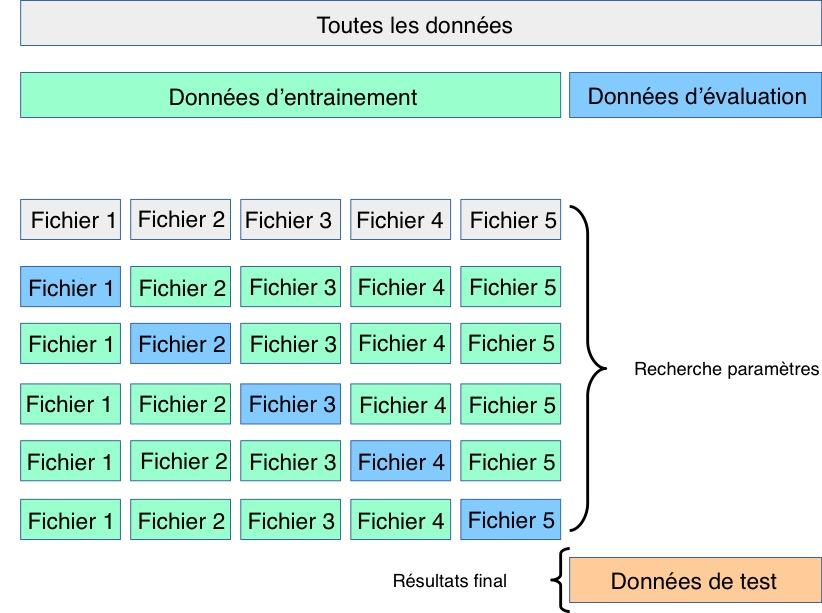
\includegraphics[scale=0.27]{gscv}
	\end{figure}
\end{frame}

\subsection{Résultats avec SVR}
\begin{frame}
	\frametitle{SVR, premier résultat}
	Approche à l'aide du modèle SVR.
	
	Noyau «\,rbf\,» $\rightarrow$ ajustement du paramètre $C$
	\begin{figure}[tc]
		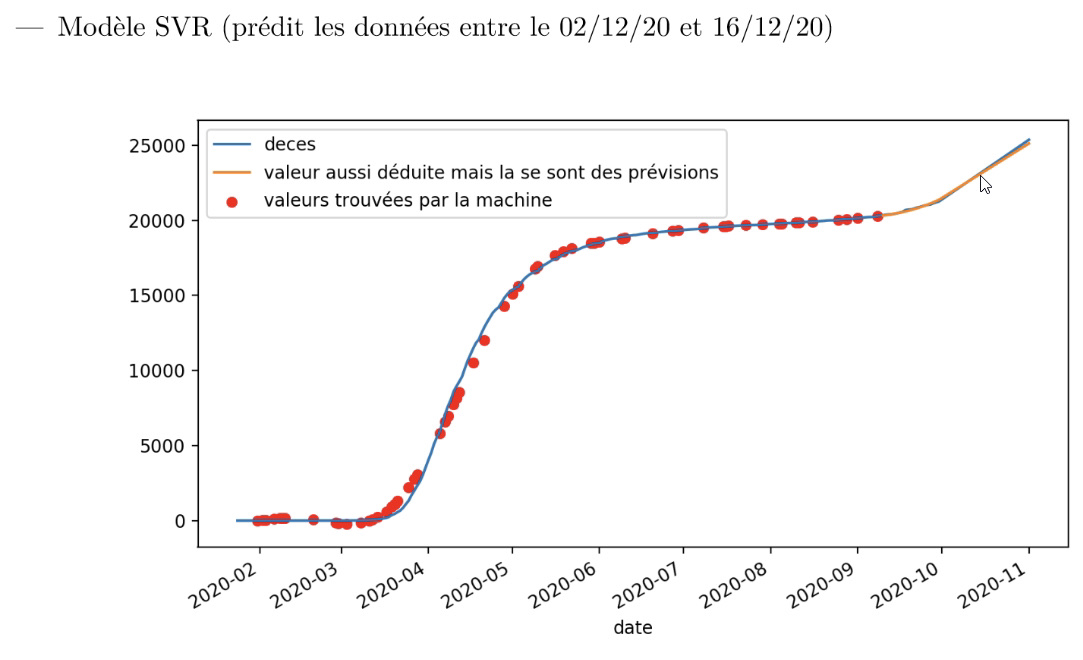
\includegraphics[scale=0.2]{SVR_premierdecoup}
		\centering
		\caption{Premier résultat avec SVR et découpage inadapté, $C=50k$}
	\end{figure}
\end{frame}

\begin{frame}
	\frametitle{Découpage adapté pour la validation croisée}
		Remise en question de la méthode de découpage
		\begin{figure}[h]
			\centering
			\begin{minipage}{0.5\textwidth}
				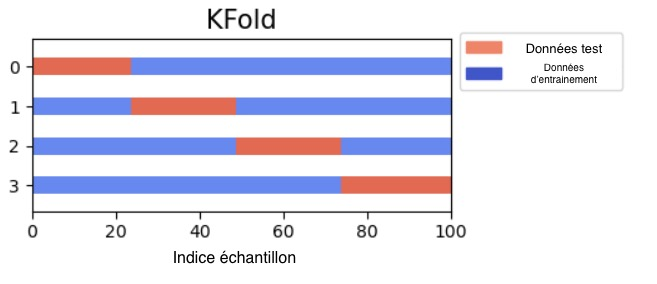
\includegraphics[scale=0.3]{kfold}
			\end{minipage}
			\centering
			\begin{minipage}{0.5\textwidth}
				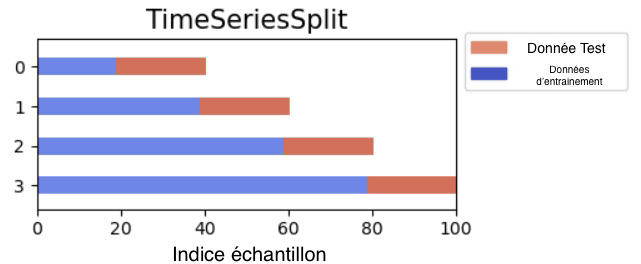
\includegraphics[scale=0.3]{tscv}
			\end{minipage}
		\caption{Comparaison des découpages pour la validation croisée}
		\end{figure}
\end{frame}

\begin{frame}
	\frametitle{SVR}
	Avec $C=10^{5}$
	\begin{figure}[t]
		\centering
		\begin{minipage}{0.4\textwidth}
			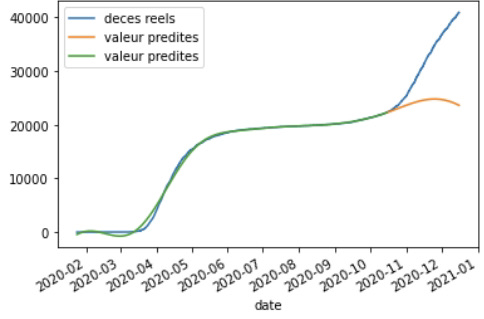
\includegraphics[scale=0.26]{SVR_avant_pt_dinflexion}
		\end{minipage}
		\begin{minipage}{0.4\textwidth}
			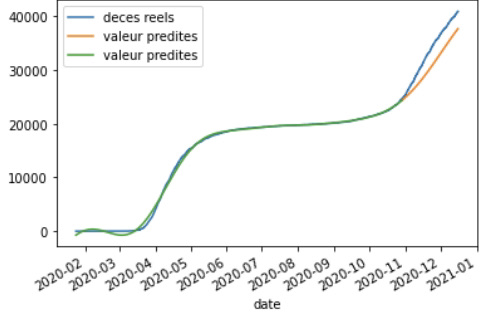
\includegraphics[scale=0.26]{SVR_apres_pt_dinflexion}
		\end{minipage}
	\caption{À gauche: prediction avant point d'inflexion; à droite: après.}
	\end{figure}
	$\Rightarrow$ Prédiction inefficace du point d'inflexion.
\end{frame}

\section{Approche multivariées}
\subsection{Multiregresseur : 'RegressorChain'}
\begin{frame}%SUPPRIMER CELUI LA?
	\frametitle{RegressorChain SVR}
	Multiregresseur RegressorChain\\ Corrélation : Cas confirmé $\rightarrow$ réanimation $\rightarrow$ décès 
	
	\begin{figure}[h]
		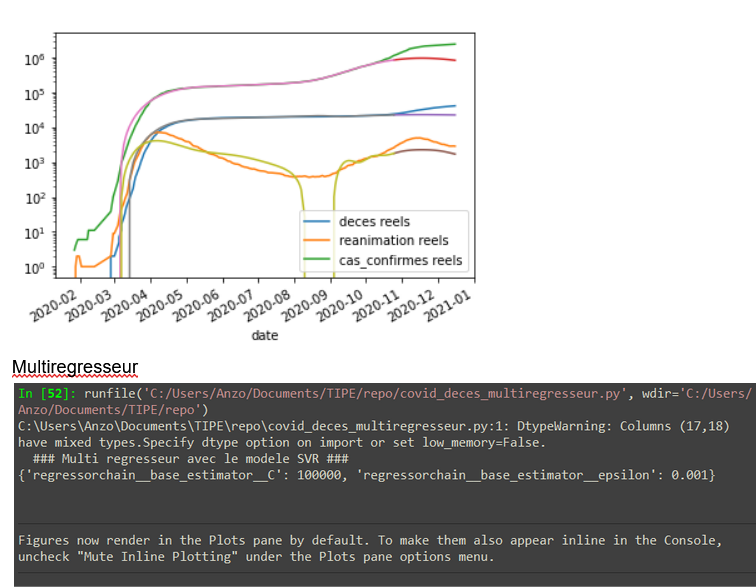
\includegraphics[scale=0.43]{mulitregr_epic_fail}
		\caption{Résultat avec SVR insatisfaisant}
	\end{figure}
\end{frame}

\begin{frame}
	\frametitle{RegressorChain TheilSenRegressor}
	Changement de régresseur : meilleurs résultats
	\begin{figure}[h]
		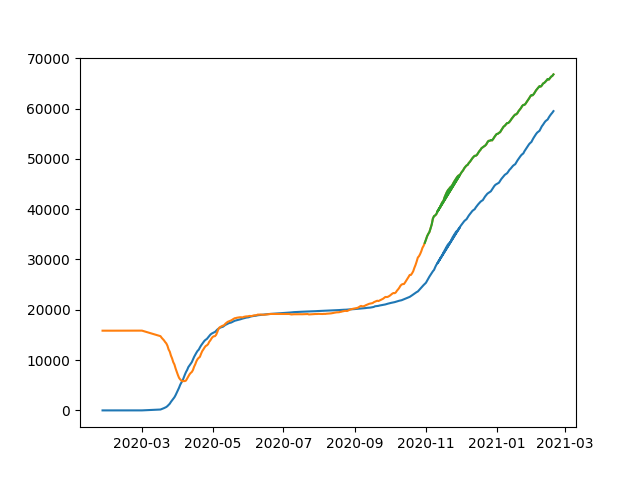
\includegraphics[scale=0.327]{theiltruc 9000 iter tol 0,001; 10 jour de plus}
		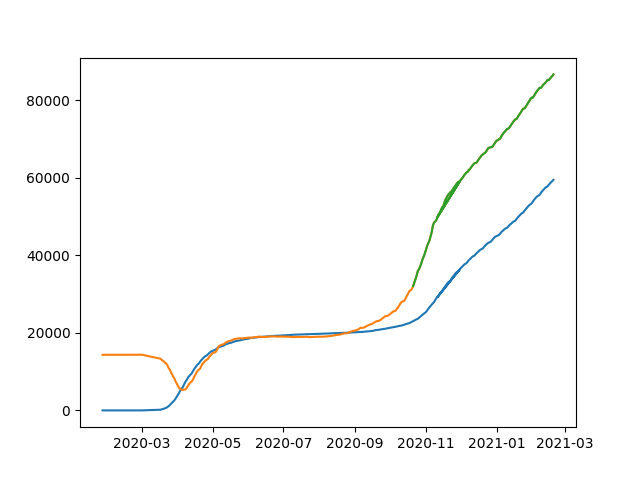
\includegraphics[scale=0.327]{theiltruc 90000 iter tol 0,001}
		\caption{Prédiction avec et sans point d'inflexion}
	\end{figure}
\end{frame}

\subsection{Réseau neuronal}
\begin{frame}
	\frametitle{Principe du réseau neuronal}
	\begin{figure}[t]
		\centering
		\begin{minipage}{0.5\textwidth}
			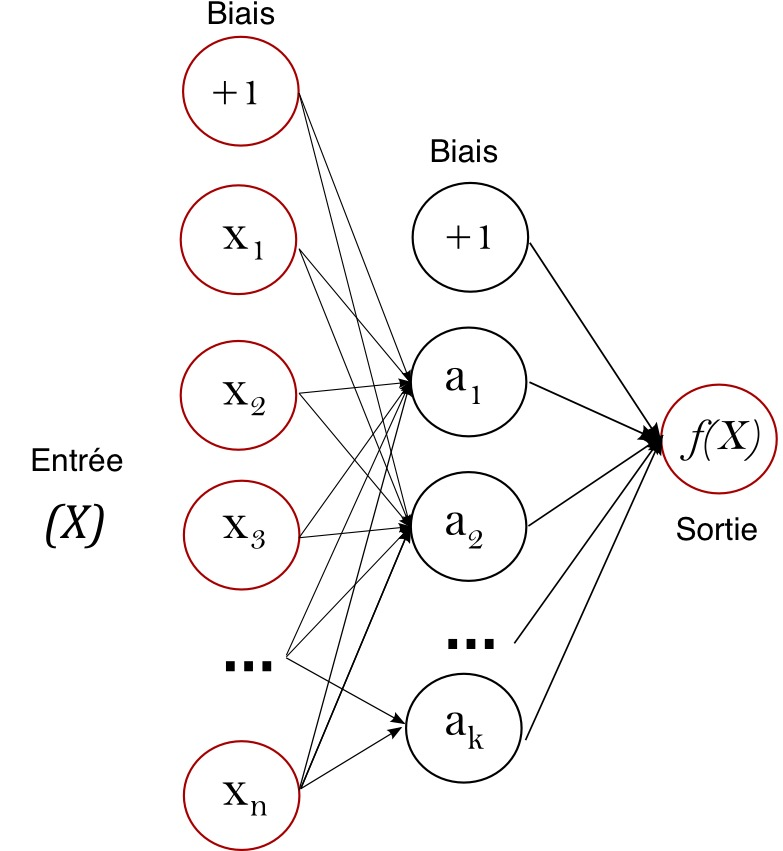
\includegraphics[scale=0.2]{nn_sk}
		\end{minipage}
	\end{figure}
\end{frame}

\begin{frame}
	\frametitle{Décalage de courbes}
	Représentation avant et aprés décalage
	\begin{figure}[h]
		\centering
		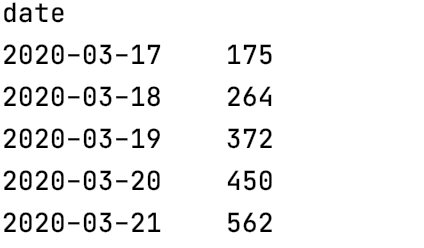
\includegraphics[scale=0.5]{decal2}
		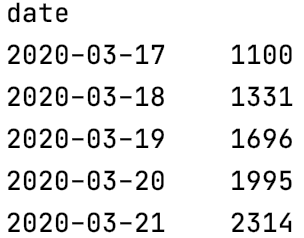
\includegraphics[scale=0.5]{decal1}
		\includegraphics[scale=0.4]{décalage 7 jour deces}
	\end{figure}
\end{frame}

\begin{frame}
	\frametitle{Corrélation et Premier résultat}
	Corrélation cas confirmés et décès : 0.978
	\begin{figure}[h]
		\centering
		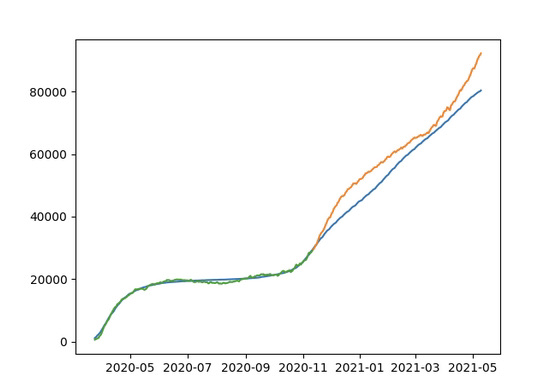
\includegraphics[width=0.46\textwidth]{NN_1}
		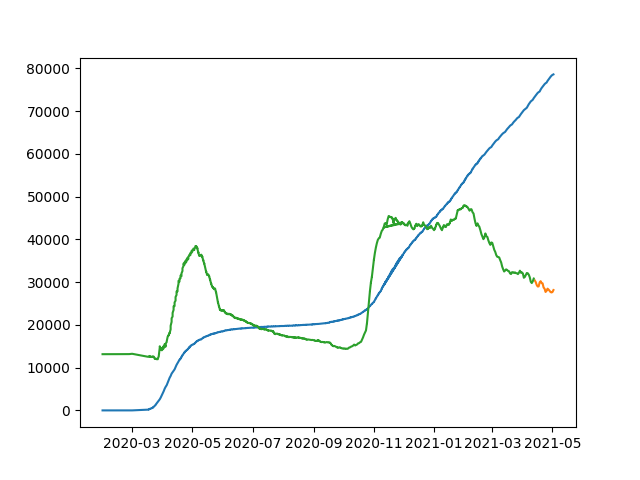
\includegraphics[width=0.4617\textwidth]{NN mlpregressor 140k iter (updated data)}
		\caption{Tests avec et sans cas confirmés}
	\end{figure}
	Échec du modèle sans les cas confirmés $\rightarrow$ cohérent avec corrélation
\end{frame}

\begin{frame}
	\frametitle{Résultats}
	Réseaux neuronaux : Meilleurs paramètres
	\begin{figure}
		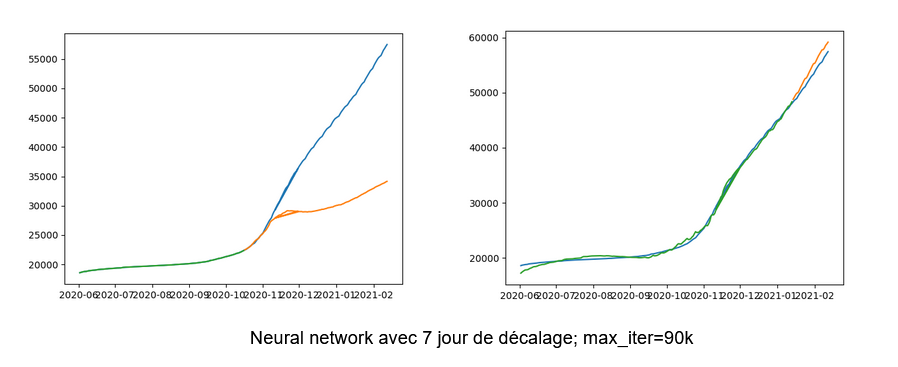
\includegraphics[scale=0.6]{NN_3}
	\end{figure}
\end{frame}

\begin{frame}
	\frametitle{Augmentation du décalage}
	Résultats insatisfaisant 
	\begin{figure}
		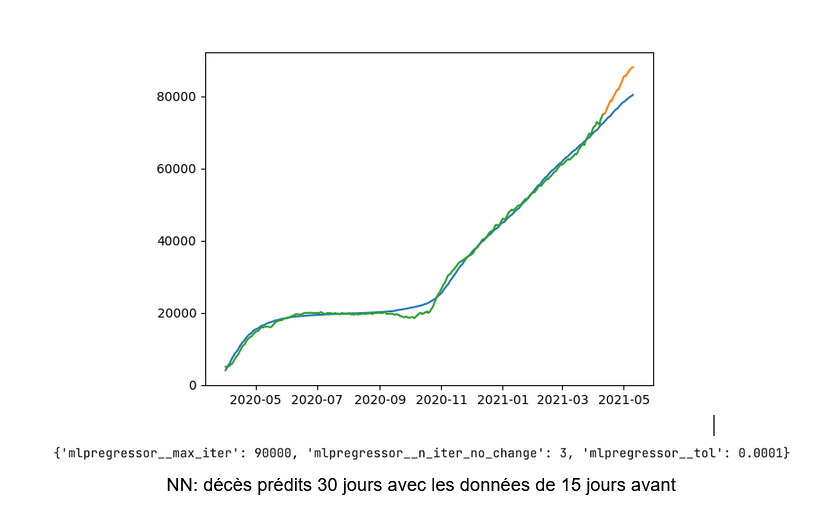
\includegraphics[width=0.7\textwidth]{NN_2}
		\caption{Tests avec 30 jour de décalage}
	\end{figure}
\end{frame}

\begin{frame}
	\frametitle{Conclusion}
	Modèle peu fiable hors situation stabilisée ou début d'évolution
\end{frame}

\appendix



\end{document}
